\chapter{彩虹表算法的优化}
%\section{计算能力优化}
\section{基于CUDA并行计算优化}
密码破解主要的瓶颈在于现有的计算能力上,假如我们目前已经拥有量子计算机的处理能力,那么现有的所有的现代加密算法都是可以短时间内被破解的,所以我们要提升破解时间,最首要的办法就是对系统的计算能力进行优化,本文将提出两个优化方案,并实现了基于GPU的优化方案。
下面两张图为EWSA(Elcomsoft Wireless Security Auditor)对无线加密算法WPA/WPA2 PSK密钥破解的数据对比和Pyrit软件在GPU上加速后的数据对比。从图中数据可以看出采用了GPU加速后的
破解速度有很明显提升。
\begin{figure}[!h]
\begin{floatrow}
\ffigbox{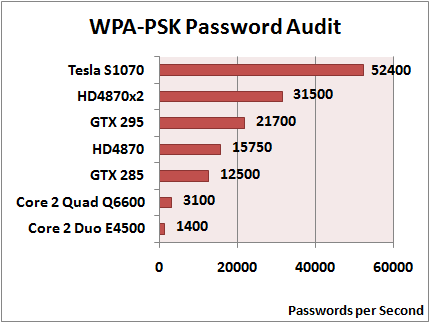
\includegraphics[scale=0.4]{ewsa}}{\caption{EWSA基于GPU加速破解WPA速度对比}}
\ffigbox{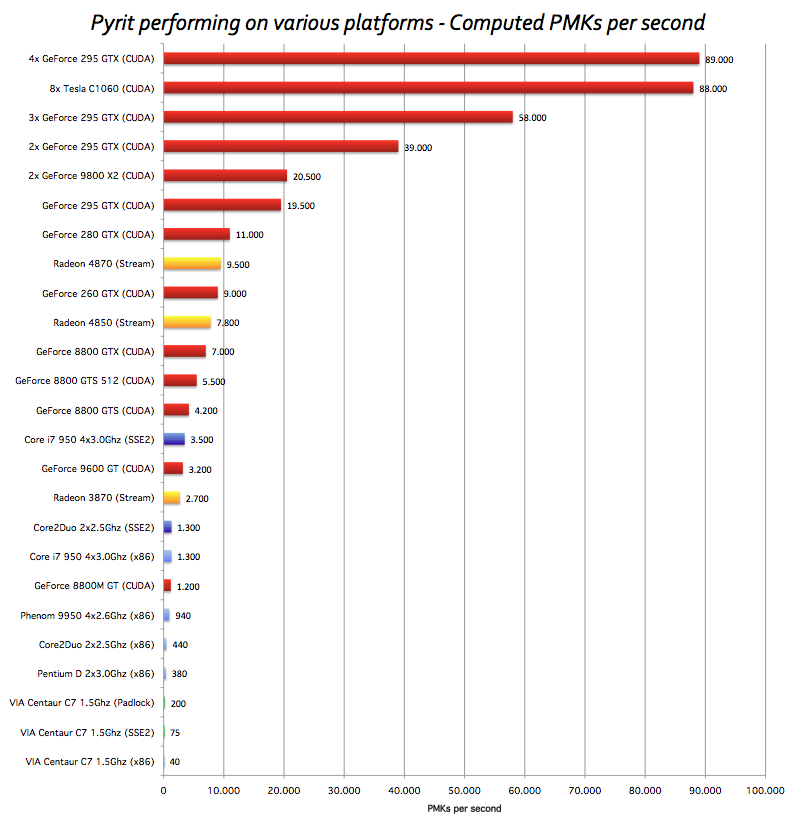
\includegraphics[scale=0.25]{pyrit}}{\caption{Pyrit基于CUDA性能测试}}
\end{floatrow}
\end{figure}

基于GPU并行计算加快破解速度会受制与显卡本身的硬件条件限制,因为每个不同型号的显卡配备的显存、寄存器、线程调度数等等都是不一样的。如何在这些局限的硬件资源上合理分配,则是GPU程序设计的关键,也是性能提升的关键。例如如何控制在同一个线程组里的线程分支数、访问全局内存的顺序都是一些常用的优化代码的方法。在实际代码设计过程中,我们首先需要将计算任务并行化,把这些并行任务分配到线程上,再由这些线程组成线程块,这些线程块将会被线程管理器动态地分配到各个流处理器进行独立的并行计算。下面我们将从GPU的硬件特性和软件特性两方面进行优化,例如减小数据传输的开销、解决共享内存的访问冲突和降低条件分支的影响等等\cite{cuda01}。
Nvidia GPU不同构架的一些规格比较,见表\ref{tab:5.2}
\begin{longtable}{@{\extracolsep{\fill}}cccc}
\caption{三代GPU间的一些规格比较}\\\toprule[1pt]
\multicolumn{1}{c}{GPU} &
\multicolumn{1}{c}{G80} &
\multicolumn{1}{c}{GT200} &
\multicolumn{1}{c}{Fermi} \\\midrule
CUDA Cores & 128 & 240 & 512 \\
双浮点数计算能力 & 无 & 30FMA & 256FMA \\
单浮点数计算能力 & 128MAD & 240MAD  & 512FMA \\
特殊功能单元(SFUs)/SM & 2 & 2 & 4 \\
Warp调度器/SM & 1 & 1 & 2 \\
共享内存/SM & 16KB & 16KB & 可配置48KB/16KB \\
L1缓存/SM & 无 & 无 & 可配置16KB/48KB \\
L2缓存 & 无 & 无 & 768KB \\
ECC内存交验 & 不支持 & 不支持 & 支持 \\
并发内核数 & 无 & 无 & 最多16 \\
地址位宽 & 32b-bit & 32-bit & 64-bit \\
\bottomrule[1pt]
\label{tab:5.2}
\end{longtable}
\subsection{减小数据传输开销}
在目前的计算机体系结构中,像显卡这样的外设一般都是通过PCI-Express总线连接到北桥芯片,再通往CPU,这和主机内存共享与CPU传输带宽。当CUP与GPU的数据频繁交换时,这个数据传输的开销将会是程序性能主要瓶颈。因此我们的程序必须尽量地减少CPU与GPU的数据交换,通常的办法有在GPU中动态生成程序所需的数据,也可以采用异步调用,使数据传输和计算能基本同时进行。
\subsection{共享内存访问冲突}
在表\ref{tab:5.2}中我们可以看到每个SM都会拥有16KB的以上的共享内存,这块共享内存的作用是存储全局内存以外的数据,也可以作为块与块之间线程交换数据的媒介。它的访问速度比寄存器慢,但要比局部内存和全局内要快一些。如果不出现访问冲突,一个线程访问共享内存的速度几乎接近访问寄存器的速度。
图\ref{fig:5.11}Fermi构架的内存体系结构,除了拥有可配置的共享内存外,还有L1和L2的高速缓存。
\begin{figure}[!ht]
\centering
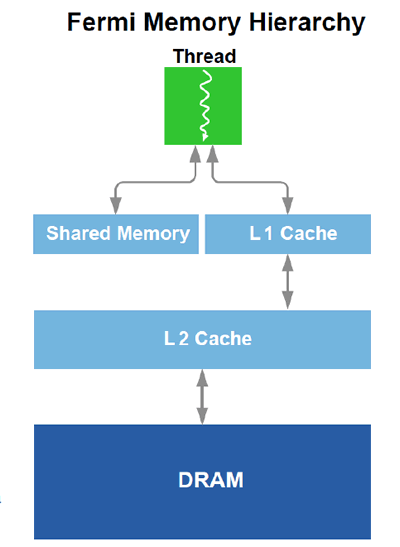
\includegraphics[scale=0.4]{fermi-memory}
\caption{Fermi构架的存储层次结构}
\label{fig:5.11}
\end{figure}
%\subsection{条件分支}
\subsection{核心配置优化}
核心程序的配置如块数、块内线程数都依赖核心代码本身,但仍然需要手工评估性能,排除大部分低效的配置。配置好块数和块内线程后,计算SM利用率,便可得到SM上活动Warp和最大Warp的比,通常我们也无需达到100\%。
\subsection{指令级别优化}
这项优化工作一般是有GPU的编译器来作的,在CUDA中是有nvcc编译器来完成的。尽量使用低延迟的指令,对全局变量或寄存器以外的局部变量,尽量少用需要多次Load和Store的操作,需要减少循环操作的开销。
\subsection{存储合并访问}
从文献\cite{cuda05}可知,SM会以时间片轮询的方式逐个调度每个Warp。各个 SM 一次只需要足够的资源以运行运行 32 个线程(通常块内线程数要远大于 32),其中的 8 个 SP 将分 4 个及其周期的时间偏离所有的线程(我们假设此处的指令为大多数可在一个周期内完成简单指令)。
当 SM 执行一条访存指令时,它首先会发出一条访存请求,并随机转向下一个就绪 Warp,而当前 Warp 将被挂起直到数据访问完成,才能再次进入就绪态并被等待属于它的时间片。理想的情况下,该 Warp 内的访存请求没有冲突,则该请求可在一个访存事务内完成。然而,事实上是否能在一个事务中结束访问,是严重依赖于 Warp内每个线程所访问存储的地址是否可合并这个事实的(Coalesced MemoryAccesses)。简单地讲,如果每个线程的访存地址是连续的,则所有 Warp 内的请求可以合并为一
个访存事务,否则将可能产生多个事务并导致该 Warp 需要更多的等待时间\cite{cuda02}。
\subsection{基于CUDA的云计算平台}
云计算是网格计算、分布式计算、并行计算、效用计算、网络存储、虚拟化、负载均衡等传统计算机和网络技术发展融合的产物。在\cite{word}一文中使用了Hadoop分布式集群优化彩虹表算法,实际上Hadoop也可以称之为一种云平台。我们也可以设计一个基于GPU加速的云计算平台,通过云平台的计算能力提升彩虹表的预运算和破解的速度。
亚马逊EC2就是这样的一个平台,它可以让用户按照自己的硬件需求租用计算机来获取计算能力。
\section{存储优化}
对于时空折中算法而言,除了要对时间进行优化,还有对空间进行优化,在不增加(或增加少量)时间代价的前提,如何减小空间代价,这就需要我们对系统进行存储优化。我们将从两方面进行改进。第一,针对存储的文件优化,也就是彩虹表文件,我们将设计一个新型的彩虹表存储结构体,减少彩虹表的磁盘存储空间,缩小系统读取文件的时间,从而提升破解的速度;第二,优化存储系统,如采用适合大文件的文件系统,采用快速的物理存储设备等方面提升读取速度。

从上一章彩虹表磁盘空间占用公式\eqref{equ:4.2}可知,想要覆盖更大的密钥空间要么增加彩虹链数或者彩虹表的张数,这都回产生庞大的彩虹表文件,可能会达到几百个GB,甚至上TB的文件,这将会增加大量的文件读取时间和磁盘空间,因此对表的存储结构进行优化将十分有必要。我们将新设计的彩虹链,在以前的存储结构中我们是使用了一个64比特的非负整形变量定义开始节点,而在实际当中,我们并不需要这么大的节点,比如在第四章中的ntlm的彩虹表中,我们只定义了26比特的开始节点和30比特的末端节点,这样一条彩虹链所占用的字节数为7Bytes。代入公式\eqref{equ:4.2}可以得到一张优化后的表的大小为448MB,优化了56.25\%。这样大大减小系统的存储空间和读取文件的时间。
\begin{figure}[!ht]
\centering
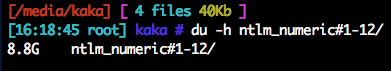
\includegraphics[scale=0.6]{5-1.png}
\caption{优化后彩虹表的空间大小}
\label{fig:5.1}
\end{figure}

新的彩虹链的数据结构实现如下,在以后的测试实验中,我们将都采用这种优化过的彩虹表。
\begin{lstlisting}
struct RTCFileHeader
{
    unsigned int   uVersion;    
    unsigned short uIndexSBits; 
    unsigned short uIndexEBits; 
    uint64         uIndexSMin;
    uint64         uIndexEMin;
    uint64         uIndexEInterval;
};
\end{lstlisting}

在存储上,除了对表的大小进行优化,还可以对系统的储存架构进行优化。在文件系统上,我们采用先进的XFS文件系统,XFS是由Silico Graphics,Inc.于90年代初开发的,它采用了优化算法,对查询分配存储空间非常快,可以支持上百万T字节的存储空间,特别是对大文件的支持表现相当出众;XFS采用B+树结构保证文件系统可以快速搜索于空间分配;XFS几乎以接近裸设备I/O的性能存储数据,在单个文件系统测试种,其吞吐量可高达7GB每秒,对单个文件的读写操作,其吞吐量可达4GB每秒。基于XFS以上特性,正符合彩虹表多个大文件读取的特点,下图为XFS与EXT3、EXT4的性能比较:
\begin{figure}[!h]
\begin{floatrow}
\ffigbox{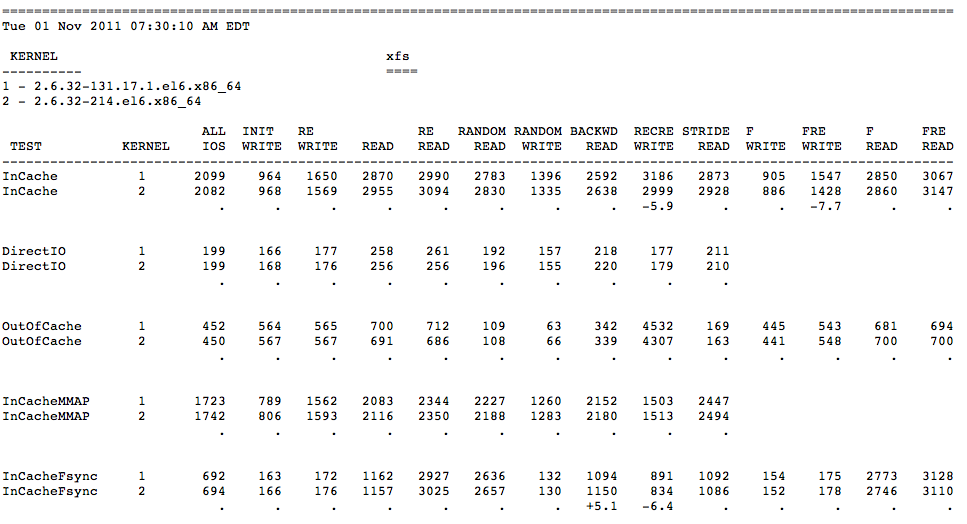
\includegraphics[scale=0.2]{5-2}}{\caption{XFS文件系统性能测试}}
\ffigbox{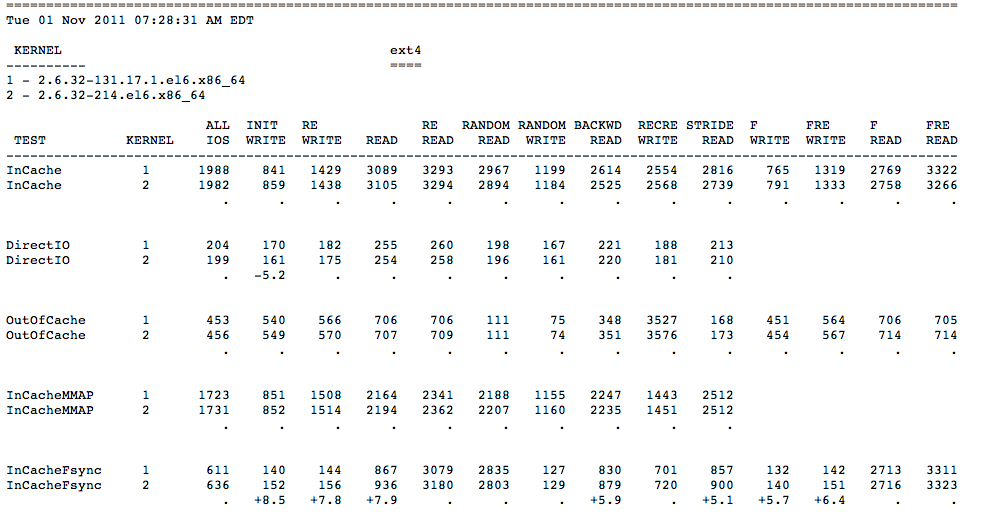
\includegraphics[scale=0.2]{5-3}}{\caption{EXT4文件系统行性能测试}}
\end{floatrow}
\end{figure}
%\begin{figure}[!ht]
%\centering
%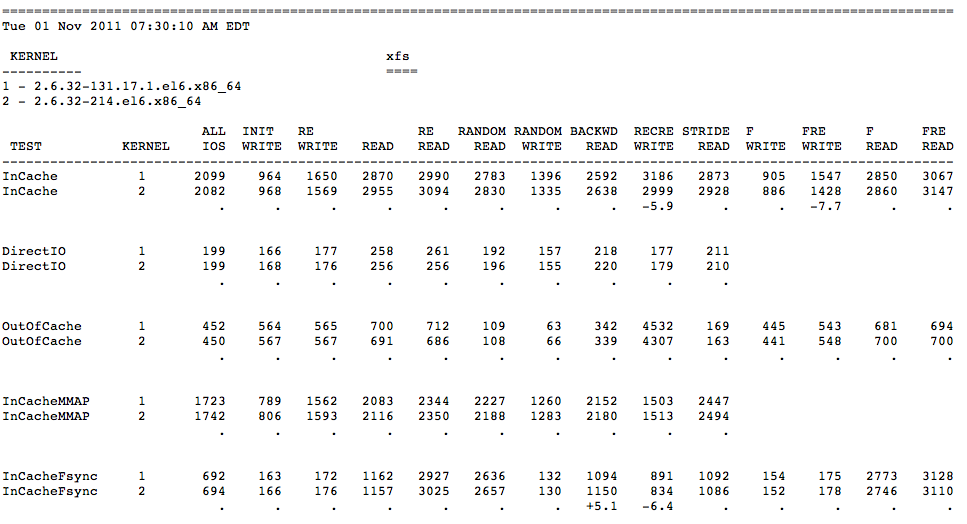
\includegraphics[scale=0.35]{5-2.png}
%\caption{XFS性能测试}
%\label{fig:5.2}
%\end{figure}
%\begin{figure}[!ht]
%\centering
%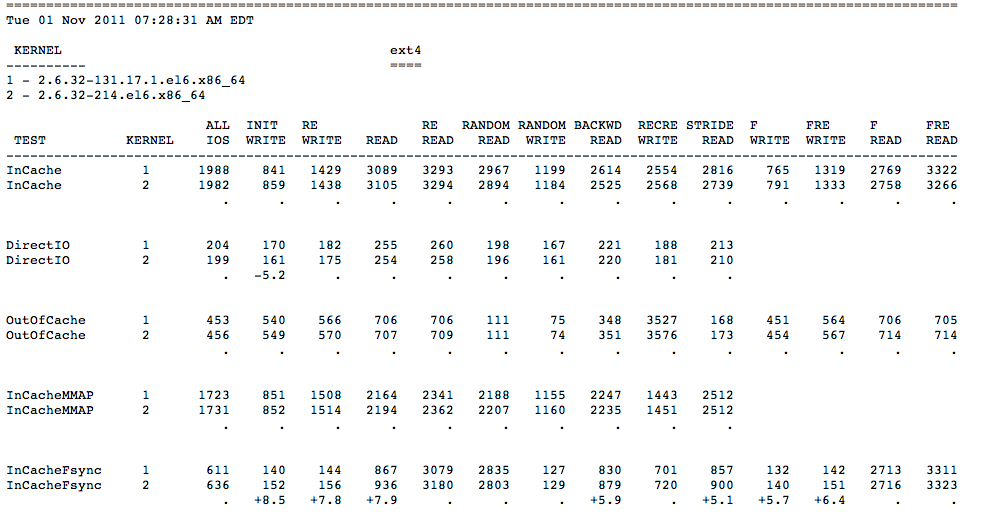
\includegraphics[scale=0.35]{5-3.png}
%\caption{EXT4性能测试}
%\end{figure}

从这上面两组性能测试数据我们可以看出XFS在大多数的的选项上要优于EXT4文件系统,特别是在大文件的读取上。

接着是对存储硬件升级,这里我们主要升级的是硬盘,下表\ref{tab:5.1}是我们对不同配置硬盘的读速度进行数据对比,从表中可以明显看出使用SSD硬盘RAID0阵列后,读取速度将比一块7200转的硬盘提升了10倍,这将大大缩小破解的实际时间。最后的需要升级的系统内存,我们知道在计算机存储体系结构中,内存的读取速度要比硬盘快上许多倍,在Linux系统上内存以/dev/shm/设备呈现给用户,用户可以对次进行读写操作。

往后我们还可以采用iSCSI网络存储结构,iSCSI技术一种优IBM公司研究开发的,是一种新存储技术,可是实现在IP网络上运行SCSI协议,使其能在高速千兆或万兆以太网上进行网络传输。再加上FCoE技术,可以达到几Gb/s的存储速度。
\begin{longtable}{@{\extracolsep{\fill}}ccc}
\caption{各种存储系统读速度对比数据}\\\toprule[1pt]
\multicolumn{1}{c}{硬盘配置} & 
\multicolumn{1}{c}{读速度(hdparm -t)} &
\multicolumn{1}{c}{索引速度} \\\midrule
1x Maxtor 6B250S0 7200 RPM & 54MB/s & 640h/s \\
6x Seagate 7200 RPM (RAID6) & 390MB/s & 4375h/s \\
2x APPLE SSD SM128C (RAID0) & 522MB/s & 6120h/s \\
\bottomrule[1pt]
\label{tab:5.1}
\end{longtable}

\section{算法结构优化}
密钥明文字符集被预计算成hash密文并和明文成对地储存在彩虹链中,如果要破解的hash密文在我们之前生成好的彩虹链中,则破解成功,反之破解失败。彩虹链存储的“明文-密文”对数量随着链表长度(t)的增加而增加,然而这些彩虹链会产生冲突,主要由于减约函数并不是一一对应的。图\ref{fig:5.5}示意了冲突的过程,最后这两条链表会合并成一条。
\begin{figure}[!ht]
\centering
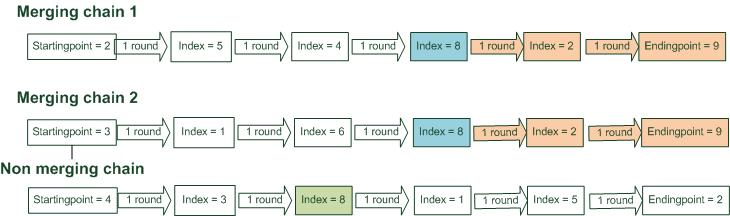
\includegraphics[scale=0.6]{5-5}
\caption{链表合并过程示意图}
\label{fig:5.5}
\end{figure}

无冲突的彩虹链个数会随着彩虹表的长度增加而减少,根据公式\eqref{equ:3.13},利用matlab软件我们可以得到关系图\ref{fig:5.6}。
\begin{figure}[!ht]
\centering
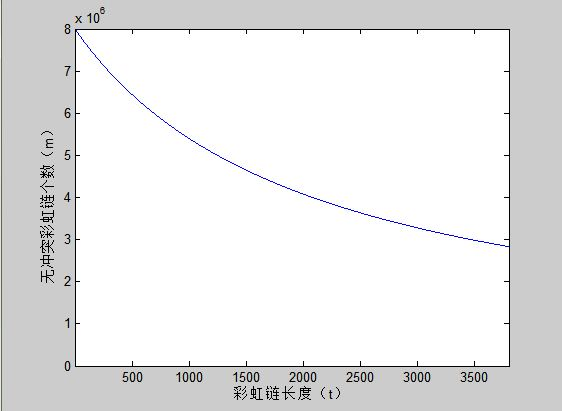
\includegraphics[scale=0.4]{5-6}
\caption{无冲突链表数-链表长度关系}
\label{fig:5.6}
\end{figure}

接着我们来分析表的张数(参数l)对破解成功概率的影响,我们把破解成功率公式\eqref{equ:3.13}在matlab下的实现函数为:\\
demo\_advantage\_of\_multiple\_table(),具体的函数实现可以参考附录A1.2。我们用不同的曲线表示当硬盘空间增大的情况下,破解的成功概率会随之增加,下图中有5条曲线,分别表示彩虹表张数为1\~5时,破解的成功率和硬盘空间之间的关系,放大后,我们可以看出彩虹表的张数越多,曲线越快接近100\%,也就是在其他参数不变的情况下,增加参数l(彩虹表张数),可以得到越高破解成功概率;但也不是生成的彩虹表张数越多越好,当随着彩虹表的增加,我们需要在存储空间也就越大,这样会破解实际所消耗的时间就会增加,反而适得其反,所以时空折中算法的精髓就在于对时间和空间的代价进行不断地平衡,找出一个折中的代价。
\begin{figure}[!h]
\begin{floatrow}
\ffigbox{\caption{5张彩虹表的破解成功率}}{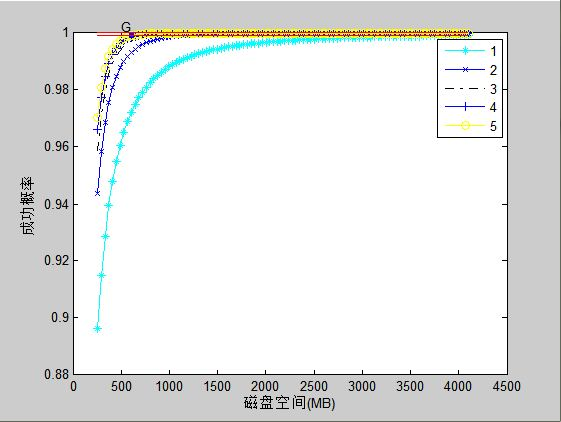
\includegraphics[scale=0.35]{5-7}}
\ffigbox{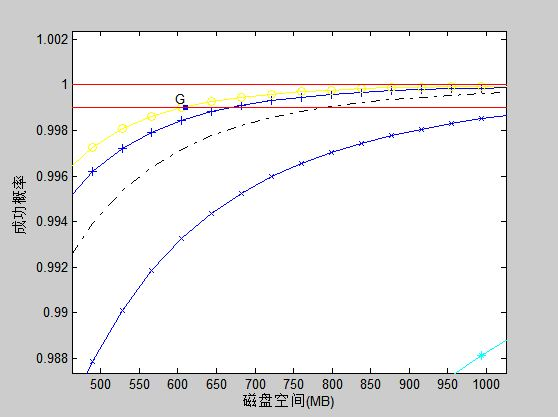
\includegraphics[scale=0.35]{5-8}}{\caption{5张彩虹表的破解成功率(放大)}}
\end{floatrow}
%\label{fig:5.7}
\end{figure}
\begin{figure}[!h]
\begin{floatrow}
\ffigbox{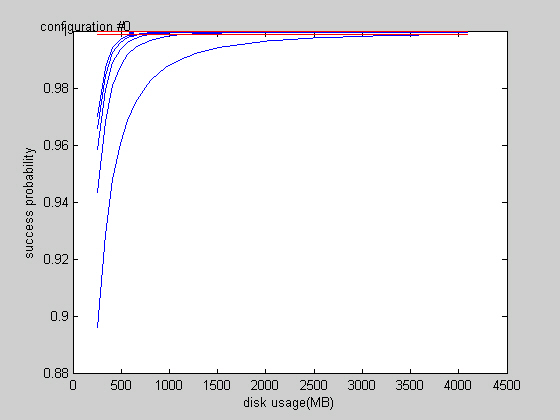
\includegraphics[scale=0.35]{5-9}}{\caption{总表空间大小-成功率关系图}}
\ffigbox{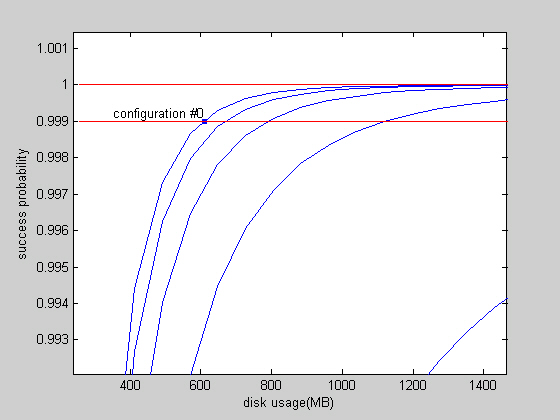
\includegraphics[scale=0.35]{5-10}}{\caption{总表空间大小-成功率关系图(放大)}}
\end{floatrow}
\end{figure}
\clearpage
\section{实验结果}
实验所用的测试平台见下表\ref{tab:5.3}:
\begin{longtable}{@{\extracolsep{\fill}}cc}
\caption{实验数据测试平台配置}\\\toprule[1pt]
\multicolumn{1}{c}{CPU} & \multicolumn{1}{c}{Intel Core i7-920 OC 4.0GHz (EIST/C1E off)} \\\hline
主板 & Asustek Rampage II GeneIntel X58芯片 \\\hline
显卡 & GeForce GTX 480 1536MB(Core/Shader/memory:700/1401/1848MHz) \\\hline
内存 & GSKILL F3-12800CL9T OC DDR3-1600 2G*3 \\\hline
硬盘 & 2x Intel 120G SSD SM128C (RAID0) \\\hline
电源 &  CougarGX 900W  \\
\bottomrule[1pt]
\label{tab:5.3}
\end{longtable}
实验方法是通过采用上述优化方法和技术,对SHA-1 、MD5和NTLM三种Hash加密算法进行实验,我们规定密钥的字符集范围(字符集对照表参见附录\ref{cha:a_c}),密钥长度,限定成功率在99.9\%以上,主要从破解时间方面针对优化前和优化后的实验数据进行对比。

在这里需要说明的是破解的时间主要分为对彩虹表文件的读取时间和密钥查表破解的时间。对彩虹表文件的读取时间主要优化方法和技术参见本章的存储优化一节,上文已经给出了基本的实验对比数据,就不在这里赘述,我们只对比最后的实际破解时间。
所有实验只针对1条Hash密文进行破解,每组彩虹表破解3次。

SHA1破解实验,破解速度提升了5.88倍,详细实验数据参考下表\ref{tab:5.5}:
\begin{longtable}{@{\extracolsep{\fill}}ccccc}
\caption{SHA1破解实验数据对比}\\\toprule[1pt]
\multicolumn{1}{c}{字符集} &
\multicolumn{1}{c}{密钥长度} &
\multicolumn{1}{c}{成功率} &
\multicolumn{1}{c}{优化前破解时间(秒)}&
\multicolumn{1}{c}{优化后破解时间(秒)}\\\midrule
\endfirsthead
\caption[]{SHA1破解实验数据对比(续)}\\
\multicolumn{5}{r}{\footnotesize 接上页}\\
\toprule[1pt]
\multicolumn{1}{c}{字符集} &
\multicolumn{1}{c}{密钥长度} &
\multicolumn{1}{c}{成功率} &
\multicolumn{1}{c}{优化前破解时间(秒)}&
\multicolumn{1}{c}{优化后破解时间(秒)}\\\endhead
numeric & 1~12 & 99.9\% & 27.54 & 4.78 \\
numeric & 1~12 & 99.9\% & 23.32 & 4.04 \\
numeric & 1~12 & 99.9\% & 36.21 & 5.98 \\\hline
loweralpha & 1~9 & 99.9\% & 21.08 & 6.76 \\
loweralpha & 1~9 & 99.9\% & 19.65 & 5.88 \\
loweralpha & 1~9 & 99.9\% & 30.18 & 8.90 \\
\bottomrule[1pt]
\label{tab:5.5}
\end{longtable}
MD5破解实验,破解速度提升了6.3倍,详细实验数据参考下表\ref{tabl:5.6}:
\begin{longtable}{@{\extracolsep{\fill}}ccccc}
\caption{MD5破解实验数据对比}\\\toprule[1pt]
\multicolumn{1}{c}{字符集} &
\multicolumn{1}{c}{密钥长度} &
\multicolumn{1}{c}{成功率} &
\multicolumn{1}{c}{优化前破解时间(秒)}&
\multicolumn{1}{c}{优化后破解时间(秒)}\\\midrule
ascii-32-95 & 1~7 & 99.9\% & 372.33 & 69.47 \\
ascii-32-95 & 1~7 & 99.9\% & 487.26 & 54.90 \\
ascii-32-95 & 1~7 & 99.9\% & 432.98 & 96.22 \\
\bottomrule[1pt]
\label{tab:5.6}
\end{longtable}
NTLM破解实验,破解速度提升了1.77倍,详细实验数据参考下表\ref{tabl:5.7}:
\begin{longtable}{@{\extracolsep{\fill}}ccccc}
\caption{NTLM破解实验数据对比}\\\toprule[1pt]
\multicolumn{1}{c}{字符集} &
\multicolumn{1}{c}{密钥长度} &
\multicolumn{1}{c}{成功率} &
\multicolumn{1}{c}{优化前破解时间(秒)}&
\multicolumn{1}{c}{优化后破解时间(秒)}\\\midrule
numeric & 1~12 & 99.9\% & 8.32 & 7.43 \\
numeric & 1~12 & 99.9\% & 10.76 & 6.90 \\
numeric & 1~12 & 99.9\% & 5.45 & 2.08 \\
\bottomrule[1pt]
\label{tab:5.7}
\end{longtable}

\section{本章小结}
本章对从计算能力到存储和彩虹表算法结构三方面进行优化和实现。在计算能力上我们提出了基于CUDA优化方法,并实现了CUDA GPU方案,从实际实验结果验证了这一设计方案;在存储系统上,我们提出了采用新型的彩虹表结构体,减少了彩虹表的磁盘存储空间,优化升级了物理的存储设备,在破解时间上得到了很好的提升;在彩虹表算法参数上,我们进行数据分析,优化了算法的参数。


